\chapter{Valutazione delle Performance}
La valutazione delle performance di un sistema(o system evaluation) è un argomento importante da dover trattare. Negli anni ci sono stati vari problemi ai sistemi che sono stati ideati, poichè o valutati in modo scorretto o progettati male. Lo scopo principale della system evaluation è quallo di misurare le prestazioni di un determinato sistema, in modo che sia anche possibile confrontare i parametri con quelli di valutazione di altri sistemi (nella maniera più oggettiva possibile).

\section{System Evaluation}
Per la system evaluation, quindi, è importante impostare e delineare un metodo formale di valutazione. Ciò ci permette di ridurre gli errori legati a particolari operazioni e di poter definire una serie di "passi" da seguire per effettuare una corretta valutazione delle performance.
In linea formale, la system evaluation si divide un due principali categorie:
\begin{itemize}
    \item \textbf{Performance Analysis}: Tale valutazione presuppone che il sistema non possa avere alcun tipo di fallimento (failure-free). Il che va a valutare solo le performance legate al suo funzionamento. (Bisogna stare attenti quando si effettua Performance Analysis di non andare a valutare in alcun modo i casi di fallimento)
    
    \item \textbf{Dependability Analysis}: Tale valutazione ci permette di valutare per quanto tempo il sistema sia in grado di funzionare e quindi anche il caso di problematiche ed errori. (tra le analisi di dependability rientra anche la \textbf{reiability}, che definisce un parametro per identificare il tempo medio in cui il sistema fallisce [System Mean Time To Failure ]
\end{itemize}

\textit{Un esempio pratico per capire i concetti di \textbf{Performance Analysis} e \textbf{Dependability Analysis} è quello di un auto di formula 1. Nel caso della Performance Analysis vado solo a valutare le specifiche performance (velocità massima, tenuta in curva, aerodinamica), senza tener conto in alcun modo di qualunque tipo di fallimento; mentre nel caso della Dependability Analysis si va a valutare quanto la macchina riesca a resistere in pista (durata delle gomme, tempo effettivo di funzionamento, casi di guasti imprevisti).
}

\subsection{Passi per la valutazione di un sistema}
Come introdotto precedentemente, per la valutazione "corretta" (o di buona qualità) di un sistema, è ottimale definire una serie di passi da seguire, in modo da redere il criterio di valutazione il quanto più formale possibile. I passi per valutare un sistema sono i seguenti:
\begin{enumerate}
    \item Definire cosa bisogna valutare
    \item Ottenere informazioni sul sistema
    \item Effettuare le misurazioni
    \item Analisi dei risultati
    \item Trovare e valutare il corretto feedback da dare sulle considerazioni iniziali
\end{enumerate}

\subsection{Performance Analysis}
Nell'analisi delle performance, quindi, si va a presupporre che il sistema di base funzioni e che quindi bisogni valutare solo il "come" tale sistema funziona (failure-free).
L'analisi delle performance può essere suddivisa formalmente in due principali parti:
\begin{itemize}
    \item \textbf{Capacity Management}: Fa in modo che le odiene risorse disponibili diano le migliori performance possibili (quindi si basa solo sulla valutazione del caso presente senza aver fatto alcuna supposizione sul carico fututo)
    \item \textbf{Capacity Planning}: Si assicura che ci sia un allocazione delle risorse in base ai workload successivi (si va a fare delle previsioni sul possibile carico futuro)
\end{itemize}

\textit{Nella spiegazione dei termini precedenti si è fatto riferimento ad una parola, ovvero \textbf{workload}. Il significato e la definizione vera e formale di workload sarà data nei capitoli successivi, per il momento possiamo definire workload come: richieste effettuate da utenti verso il sistema
}
\\\\
La Capacity Management e la Capacity Planning sono strutturate principalmente in 5 passi che portano alla corretta esecuzione della propria valutazione [\ref{img:passi}]

\begin{figure}
    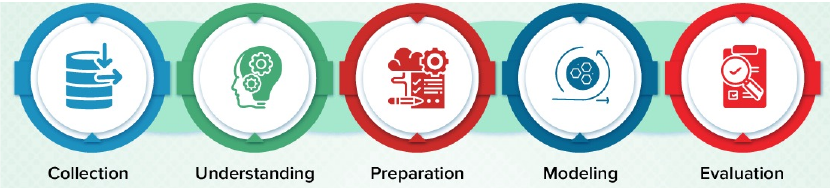
\includegraphics[width=.8\textwidth]{img/passi_CMCP.png}
    \centering
    \caption{Passi da effettuare per la CM e la CP}\label{img:passi}
\end{figure}

\subsection{Errori comuni nella System Evaluation}
Quando si fa systema evaluation, solitamente, si possono commettere degli errori, che possono portare poi ad avere uno scorretto parametro di confronto o giudizio del sistema. Gli errori che principalmente vengono fatti sono:
\begin{itemize}
  \item \textbf{Nessun obiettivo}: senza obiettivi chiari non esiste un modello universale; 
  gli obiettivi determinano tecniche, metriche e workload da usare, e non sono mai banali.
  
  \item \textbf{Obiettivi distorti}: porsi come obiettivo. Dimostrare che il nostro sistema è 
  migliore di un altro porta a una valutazione di parte, in cui gli analisti fanno da giudici invece che da osservatori imparziali.
  
  \item \textbf{Approccio non sistematico}: condurre la valutazione senza un metodo strutturato 
  (obiettivi $\rightarrow$ metriche $\rightarrow$ workload $\rightarrow$ esperimenti $\rightarrow$ analisi) 
  porta a risultati incompleti o non riproducibili.
  
  \item \textbf{Analisi senza capire il problema}: raccogliere dati e produrre grafici senza 
  aver compreso a fondo la natura del problema significa ottenere informazioni non utili alle decisioni.
  
  \item \textbf{Metriche di performance scorrette}: scegliere metriche che non riflettono gli 
  aspetti importanti del sistema (es. guardare solo il throughput quando è cruciale la latenza) porta a conclusioni fuorvianti.
  
  \item \textbf{Workload non rappresentativo}: utilizzare un carico artificiale che non riproduce 
  il comportamento reale degli utenti (picchi, mix di richieste, distribuzioni) rende i risultati poco affidabili.
  
  \item \textbf{Tecnica di valutazione sbagliata}: adottare un metodo inadeguato (analisi analitica, simulazione o misurazioni reali) 
  rispetto agli obiettivi porta a risultati poco significativi o addirittura falsati.
\end{itemize}

Dati tali errori di valutazione si comprende il motivo a cui è legato il bisogno di definire un path formale per la performance evaluation. Pertanto si va a definire una serie di passi sistematici che ci spiega come poter realizzare la syustem evaluation senza andare in contro alle problematiche descritte in precedenza. I passi da seguire sono i seguenti:
\begin{enumerate}
  \item Definire gli obiettivi e descrivere il sistema
  \item Elencare i servizi e i risultati attesi
  \item Selezionare le metriche
  \item Elencare i parametri
  \item Selezionare i fattori da studiare
  \item Scegliere la tecnica di valutazione
  \item Selezionare il workload
  \item Progettare gli esperimenti
  \item Analizzare e interpretare i dati
  \item Presentare i risultati
  \item Ripetere il processo
\end{enumerate}

Guardando tali passi si comprende che bisogna effettuare alcune scelte fondamentali. Le scelte che principalmente bisogna effettuare sono legate a: Tecniche di valutazione, Metriche di performance e Performance richieste

\subsubsection{Tecniche di valutazione}
Per valutare le performance di un sistema si possono utilizzare diverse tecniche che racchiudono una metodologia differente di approccio rispetto al sistema, che ci permette di poter valutare le prestazioni prescindendo dal sistema stesso (o in parte). Le tecniche principali di valutazione sono:
\begin{itemize}
    \item \textbf{Modellazione Analitica}: Si va a ricostruire il sistema mediante un modello matematico. Tale tecnica permette di avere una soluzione in forma chiusa (utilizza formule matematiche senza dover simulare o replicare un sistema). Tali sistemi, però, fanno delle assunzioni sul sistema, che permettono la semplificazione e la modellazione matematica
    
    \item \textbf{Simulazione}: Tale tecnica cerca di combinare la modellazione analitica del sistema con il mondo reale, cercando di emulare quanto più è possibile il caso reale tramite particolati software. \uppercase{è} una buona soluzione, poichè richiede un costo intermedio per essere effettuata; se non fosse per il tempo che bisogna dedicargli per la ricostruzione del sistema
    
    \item \textbf{Misura}: Si vanno a valutare le performance con misurazioni sul sistema reale. Tale approccio è il più costoso, sia in termini di carico che di costo, ma è il più efficiente poichè si è a contatto con il caso reale effettivo
\end{itemize}

Per selezionare la tecnica adatta al nostro caso bisogna fare una valutazione completa del sistema cercando quella che è la tecnica più adatta in base al nostro criterio di valutazione richiesto. Talvolta può essere anche possibile utilizzare più tecniche insieme. (Un esempio potrebbero essere i Twin Systems, dove vado ad effettuare modifiche prima in simulazione, e se noto miglioramento delle performance applico le stesse scelte anche al sistema reale andando ad analizzare ulteriormente le performance).

\subsubsection{Selezione della metrica}
Altro parametro importante da scegliere è la metrica da utilizzare. \uppercase{è} importante capire il corretto modo di scegliere una metrica dato che è il concetto su cui si basa il confronto tra vari sistemi. Le metriche possono basarsi su diversi criteri, i principali possono essere classificati come:
\begin{itemize}
    \item \textbf{Metriche per le performance}: Si vanno a valutare dei parametri di valutazione discreti (non probabilistici), dipendenti da: Tempo, Processing Rate, Consumo di risorse ecc.
    
    \item \textbf{Metriche per la Dependability}: Si va a valutare un sistema in base alla sua "efficenza", vista nel senso di probabilità di diversi eventi (guasti, eccezioni ecc.), esempi di tali metriche sono: Availability, Performability, Reliability ecc.
     
    \item \textbf{Metriche per i costi}: Si basano i criteri sui costi impiegati per l'implementazione di particolari sistemi
\end{itemize}

Uno dei criteri di selezione della metrica è quello presentato nell immagine [\ref{img:criterio-metrica}], che ci permette di capire, in base a come reagisci il sistema, quale tipologia e quale classe di parametri andare a considerare. Fare attenzione all'immagine, essa suddivide le possibili metriche in tre macroaree, la prima è quella riguardanti le metriche deterministiche, ovvero quelle metriche che vengono valutate su casi effettivi e risultati non di natura probabilistica; a differenza delle altre 2 categorie che, avendo a che fare con errori ecc., ricadono nei casi di dover andare a valutare il sistema mediante dei valori di natura probabilistica.

\begin{figure}
    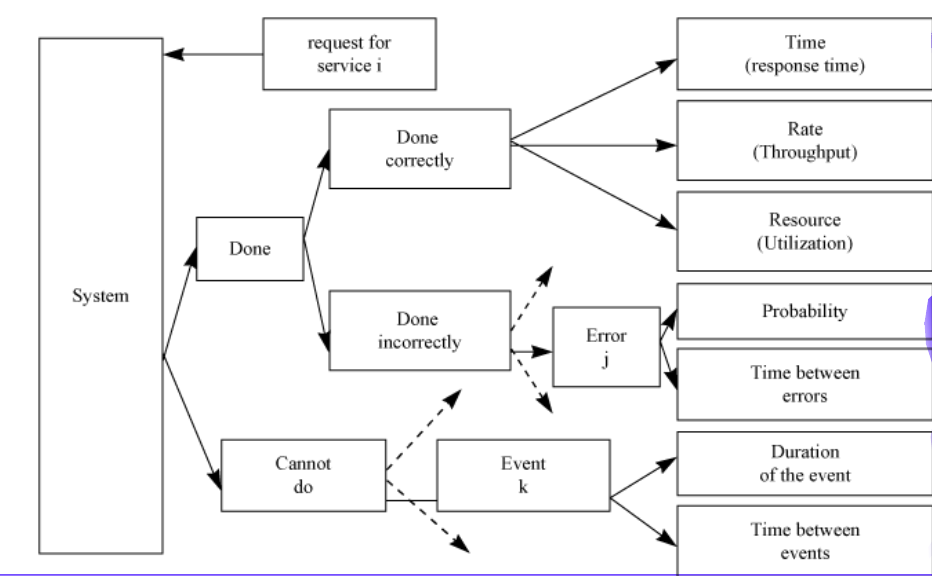
\includegraphics[width=.8\textwidth]{img/Metrics.png}
    \centering
    \caption{Criterio di selezione della metrica}\label{img:criterio-metrica}
\end{figure}

Le metriche presentate, quindi, sono le seguenti:
\begin{itemize}
    \item \textbf{Response Time}: Tale parametro ci permette di capire ogni quanto di tempo un sistema produce un risultato valido. Per la valutazione di tale parametro, però, possono essere effettuate varie tipologie di valutazione:
    \begin{itemize}
        \item \textbf{Response time}: Misurazione basata sul tempo tra l'inizio e la fine della richiesta
            
        \item \textbf{Reaction time:} Fine della richiesta dall'inizio del suo processamento
        
        \item \textbf{Turnaround time:} Inizio della richiesta fino alla fine della risposta
    \end{itemize}

    Generalmente la Response Time cresce all'aumentare del carico sul sistema, per tale caso è stato definito quello che verrà chiamato \textbf{Strech Factor} (permette di capire quando non saranno più usabili un certo numero di risorse)

    \item \textbf{Processing Rate}: Il processing rate non rappresenta altro che il throughput associato al mio sistema, e che quindi calcola la quantità di lavoro svolto da un singolo componente per unitò di tempo.
\end{itemize}

Talvolta, utilizzare sia il thoroughput che il response time può risultare ridondante, pertanto si decide di utilizzare un unico parametro, dipendente da entrambi, chiamato \textbf{potenza}, che si può calcolare come \textbf{\(\frac{Throughput}{Response Time}\)}. Pertanto è giusto andare a ridefinire anche i diversi punti di evoluzione della potenza, che racciudono la nostra attenzione

\begin{itemize}
    \item \textbf{Capacità nominale:} Rappresenta il throughput massimo raggiungibile in condizioni di carico di lavoro ideali. Tuttavia, a questo livello di throughput, il tempo di risposta è generalmente troppo elevato.
    \item \textbf{Capacità utilizzabile:} È il throughput massimo che si può ottenere, quindi è il punto massimo dopo il quale il sistema potrebbe andare in crash (quindi ad esempio ha tempi di risposta molto lunghi ma riesce a gestire molto più carico)
    \item \textbf{Capacità di "ginocchio":} È il punto operativo ottimale, considerato il miglior equilibrio tra un alto throughput e un basso tempo di risposta. Questo punto corrisponde al valore massimo della metrica Power.
\end{itemize}

Oltre la potenza un ulteriore parametro utile è la \textbf{fairness}, che ci permette di capire se un aprticolare sistema distribuisce bene il carico o meno. Ciò lo veniamo a scoprire mediante il calcolo del preciso valore di fairness che è normalizzato, e quindi compreso tra 0 ed 1.

A livello formale, si definisce:

\begin{itemize}
    \item \(x_i\), frazione del throughput associato ad \(x_i\)
    \item n, numero di utenti nel sistema
\end{itemize}

A questo punto comprendo se sto usando il throughput in maniera fair, calcolando la \textbf{fairness}, che mi dice che se ogni utente ha a disposizione una porzione eguale di throughput, allora sarà 1, mentre nel caso opposto sarà vicino allo 0.
Per calcolare la fairness si utilizza la seguente formula:

\[
fairness = \frac{\left(\sum_{i=1}^{n}x_i\right)^2}{n\sum_{i=1}^{n}x_i^2}
\]

% \[
% % fairness = \frac{\sum_{1}^{n-1}{(x_i)^2}}
% \]